\exercisetitle{
En  el  circuito  de  la  figura,  alimentado  con  un  generador  de  alterna  con  amplitud 10V,  fase  nula,  e impedancia  de  generador  $50 \Omega$,  determine  la  potencia  media  disipada  por  la  impedancia  de  carga $Z_1$. Todas las líneas de transmisión tienen impedancia característica $Z_0=50 \Omega$.
}

Para realizar este ejercicio empezaremos calculando la impedanciade entrada al sistema completo.
\subsection{Rama $Z_1$}
La impedancia se encuentra en paralelo con un stub $0.08\lambda$, por lo que calcularemos la admitancia de ambos componentes y los sumaremos:

\begin{align*}
&  Y_{stub} &=& -j \frac{1}{Z_0 \tan{\beta l}} &=& -j0.0363 \Omega \\
&  Y_L && &=& 0.019 +3.8 4 \times 10^{-3} \Omega \\
&  Y_{A} &=& Y_{stub} + Y_L &=& 0.019 -j0.032\Omega \\
&  y_{a} &=& Y_{A} / Y_{0} &=& 0.96 -j1.62 \Omega
\end{align*}

Y ahora nos iremos a la carta de smith para mover la admitancia $\lambda$ hacia el generador
\begin{figure}[h]
  \centering
  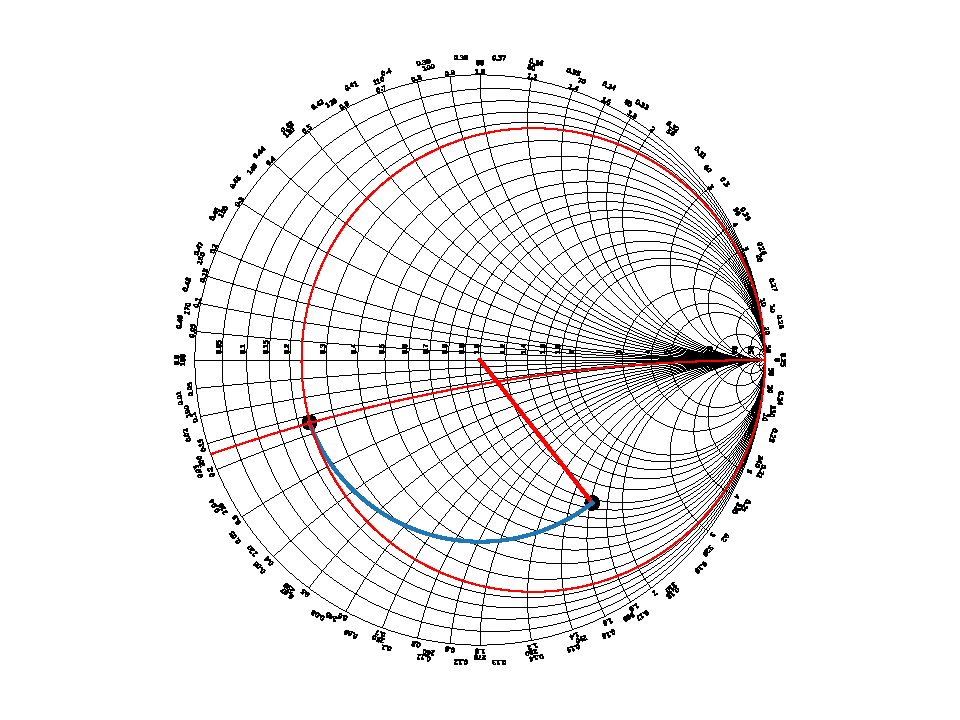
\includegraphics[scale = 0.75]{ej10/images/out1.pdf}
  \label{ej2smith}
\end{figure}

Donde comprobamos que la admitancia en ese punto para la rama $y_{r1} = 0.23 - 0.17j$. (Como todas las líneas tienen la misma impedancia característica, no tenemos porque denormalizar hasta el final)

\subsection{Rama $Z_2$}
Haremos lo mismo que se hizo en la anterior rama, pero podemos fijarnos en un detalla, la línea es de $0.25\lambda$, lo que significa que avanzaremos $\pi$ en la carta, si avanzamos otro $\pi$ para convertir a admitancia, daremos una vuelta completa, $2\pi$, por lo que podemos decir que la admitancia de entrada a la rama $Y_2$ es $5+j20 S$ que normalizado es $y_{r2} =0.1 + 0.4j$.

\subsection{Stub}
Primero necesitamos calcular la suma de las admitancias de las dos ramas, que resulta
$0.33 + 0.23j$, avanzaremos esta líneza $0.1\lambda$ y le sumaremos la admitancia delstub en paralelo, cuya admitancia normalizada es:
\[ y_{stub} = -j Z_0 \times \frac{1}{Z_0 \tan{\beta l}} = -j1.37 \]
Después avanzaremos la línea otros $0.15\lambda$ para obtener finalmente la admitancia de entrada. Estos movimientos se ven en la siguiente carta:
\begin{figure}[h]
  \centering
  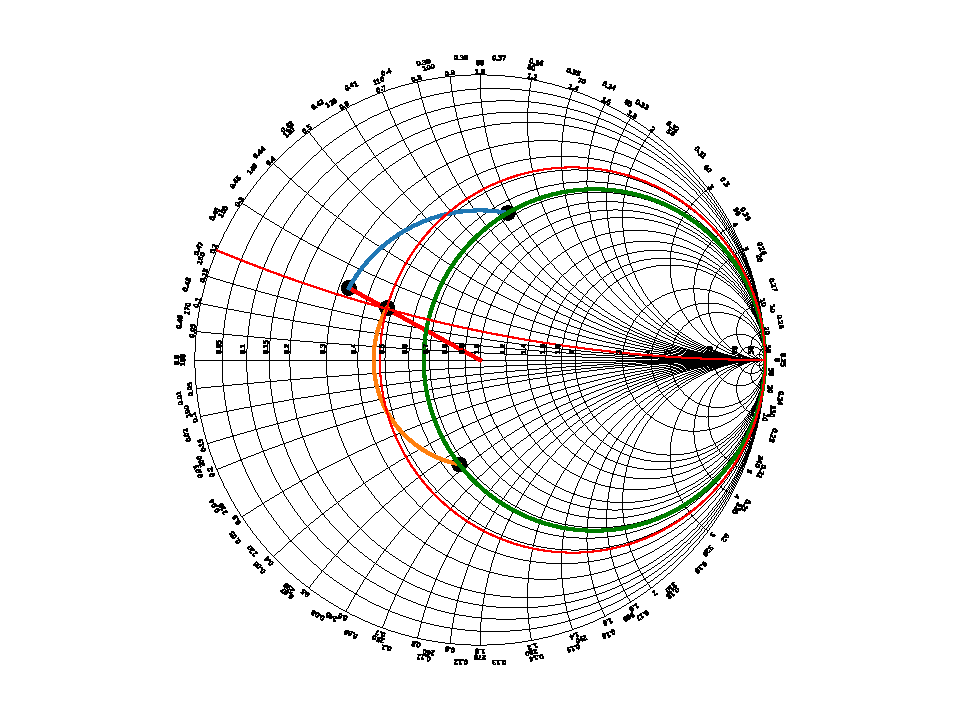
\includegraphics[scale = 0.75]{ej10/images/out2.pdf}
  \label{ej2smith}
\end{figure}
Donde podemos ver que al final obtenemos una admitancia de entrada de $y_{in} = 0.48 - j0.17$, que traducido a impedancia resulta $1.85 + j0.65$, que al denormalizar resulta:
\[Z_{in} =92.5 + j32\Omega \]

\subsection{Potencia entregada a $Z_1$}
Para ello, empezaremos calculando el voltaje de entrada:
\[V_{in} = V_S \frac{Z_{in}}{Z_S + Z_{in} } = 6.7e^{j0.114}\]
Este voltaje será el mismo a través de la línea, hasta que llegue hasta las ramas 1 y 2, ya que no hay perdidas, por tanto:
\begin{align*}
  P_{in} &= \frac{1}{2} |V_{in} |^2 \Re (\frac{1}{Z_{r1}^*})\\
  P_{in} &= \frac{1}{2} |V_{in} |^2 \Re ({Y_{r1}^*}) \\
  P_{in} &= 0.23 W
\end{align*}
